\section{Modern mixed-integer linear programming solvers}

In this chapter, we will discuss some of the numerous features that a shared by most professional-grade implementation of mixed-integer programming (MIP) solver. As it will become clear, MIP solvers are formed by an intricate collection of techniques that have been developed through the last few decades. The continuous improvement and development of new such techniques have enabled performance improvements beyond purely hardware performance progress. In fact, this is a very lively and exciting research are, with new features being proposed and incorporated in these solvers with new releases of these tools.

The main difference between MIP solver implementations is which ``tricks'' and techniques they have implemented. In some cases, these are not disclosed in full detail, since the high-performing solvers are commercial products subject to trade secrets. Luckily, some open-source and free to use alternatives have been made available, but they are not up to par with commercial implementations in terms of performance.

We will focus on describing the most important techniques forming a professional-grade MIP solver implementation. Most MIP solvers allow for significant tuning and toggling of these techniques. Therefore, knowing the most important techniques and how they work can be beneficial in configuring MIP solvers to your own needs.

Most MIP solvers implement a method that is called \emph{branch-and-cut} which consists of a combination of the LP-based branch-and-bound method (as described in Chapter \ref{chapter_9}) and a cutting-plane method (as described in Chapter \ref{chapter_10}) that is employed at the root note (or the first LP relaxation subproblem) and possibly at later nodes as well. Figure \ref{p1c11:fig:MIP_solver_flowchart} illustrates the typical flowchart of a MIP solver algorithm.

\begin{figure}
	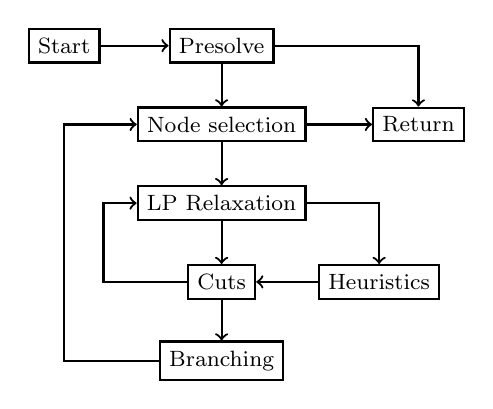
\begin{tikzpicture}[scale=1, node/.style={draw, thick, font=\footnotesize}]
		\node[node] (Start) at (0,6) {Start};
		\node[node] (Presolve) at (2,6) {Presolve};
		\node[node] (Return) at (4.5,5) {Return};
		\node[node] (Node selection) at (2,5) {Node selection};
		\node[node] (LP relaxation) at (2,4) {LP Relaxation};
		\node[node] (Cuts) at (2,3) {Cuts};
		\node[node] (Branching) at (2,2) {Branching};
		\node[node] (Heuristics) at (4,3) {Heuristics};
		% Arrows
		\draw[thick, ->] (Start) --(Presolve);
		\draw[thick, ->] (Presolve) -- (Node selection);
		\draw[thick, ->] (Presolve) -- (4.5,6) -- (Return);
		\draw[thick, ->] (Node selection) -- (LP relaxation);
		\draw[thick, ->] (Node selection) -- (Return);
		\draw[thick, ->] (LP relaxation) -- (Cuts);
		\draw[thick, ->] (LP relaxation) -- (4,4) -- (Heuristics);
		\draw[thick, ->] (Cuts) -- (Branching);
		\draw[thick, ->] (Heuristics) -- (Cuts);
		\draw[thick, ->] (Branching) -- (0,2) -- (0,5) --(Node selection);
		\draw[thick, ->] (Cuts) -- (0.5,3) -- (0.5,4) -- (LP relaxation);
	\end{tikzpicture} 
	\caption{The flowchart of a typical MIP solver. The nodes represent phases of the algorithm} \label{p1c11:fig:MIP_solver_flowchart}
\end{figure}

The first phase consists of a preprocessing phase called \emph{presolve}. In that, the problem formulation is analysed to check whether redundant constraints or loose variables can be trivially removed. In addition, more sophisticated techniques can be employed to try to infer the optimal value of some variables via logic or to tighten their bounds. For simple enough problems, the presolve might be capable of returning an optimal solution or a certificate that the problem is infeasible or unbounded.

Then, the main solution loop starts, similarly to what we have described in Chapter \ref{chapter_9} when discussing the branch-and-bound method. A node selection method is employed and the LP relaxation is solved. Then, branching is applied and the process continues until an optimal solution has been found. 

The main difference however relates to the extra \emph{Cuts} and \emph{Heuristics} phases. Together with the \emph{Presolve}, this is likely the phases that most differ between implementations of MIP solvers. The cut phase consists of the employment of a cutting-plane method onto the current LP relaxation with the aim of either obtaining an integer solution (and thus pruning the branch by optimality) or strengthening the formulation of the LP relaxation, as discussed in Chapter \ref{chapter_10}. Each solver will have their own family of cuts that is used in this phase, and typically a collection of them are used simultaneously. The heuristics phase is used in combination to try to obtain primal feasible solutions from the LP relaxations (possibly augmented by cuts) so primal bounds can be obtained and broadcast to the whole search tree, hopefully fostering pruning by bound. 

In what follows, we will discuss the main techniques in each of these phases. 


\section{Presolving methods}

Presolving (or preprocessing) methods are methods typically employed before the start of the branch-and-cut method. These methods have three main goals: (i) reducing the problem size by fixing variables and eliminating constraints; (ii) strengthening the LP relaxation by identifying bounds and coefficients that can be tightened; and (iii) exploit integrality to improve formulation and identify problem structures (e.g., knapsack or assignment structures)


\subsubsection{Detecting infeasibility and redundancy}

Many techniques used in the preprocessing phase relies on the notion of constraint activity. Consider the constraint $a^\top x \leq b$, with $x \in \reals^n$ as a decision variable vector, $l \leq x \leq u$, $b \in \reals$, where $(a,b,l,u)$ are given. We say that the \emph{minimum activity} of the constraint is given by
%
\begin{equation*}
	\alpha_{\text{min}} = \min\braces{a^\top x : l \leq x \leq u} = \sum_{j : a_j > 0}a_jl_j + \sum_{j : a_j < 0}a_j u_j.	
\end{equation*}
%
Analogously, the \emph{maximum activity} of a constraint is given by 
%
\begin{equation*}
	\alpha_{\text{max}} \hspace{-2pt} = \max\braces{a^\top x : l \leq x \leq u} = \sum_{j : a_j > 0}a_ju_j + \sum_{j : a_j < 0}a_jl_j
\end{equation*}

This constraint activity can be used in number of ways. For example, if there is a constraint for which $\alpha_{\text{min}} > b$, then the problem is trivially \emph{infeasible}. On the other hand, if one observes that $\alpha_{\text{max}} \leq b$ for a given constraint, then the constraint can be safely removed since it is guaranteed to be redundant.


\subsubsection{Bound tightening}

Another important presolving method is bound tightening, which, as the name suggests, tries to tighten lower and upper bounds of variables, thus strengthening the LP relaxation formulation. There are alternative ways that this can be done, and they typically trade off how tightening can be observed and how much computational effort they require. 

One simple way of employing bound tightening is by noticing the following. Assume, for simplicity, that $a_j > 0$. Then, we have that
%
\begin{equation*}
	a^\top x \leq b \Rightarrow 
	a^\top x - a_jx_j + a_jx_j \leq b \Rightarrow
	x_j \leq \frac{b - (a^\top x - a_jx_j)}{a_j},	
\end{equation*}
%
which must also hold for 
%
\begin{equation*}
	x_j \leq \frac{b - \alpha_{\text{min}} + a_jl_j}{a_j},
\end{equation*}
%
in turn, yield an upper bound for $x_j$. The procedure can be analogously adapted to obtain a lower bound as well. Furthermore, rounding can be employed in the presence of integer variables. 

Another common bound technique consists of solving a linear programming subproblem for each variable variable $x_j$, $j =1, \dots, n$. Let
%
\begin{equation*}
	IP : \mini \braces{c^\top x : x \in X = P \cap \integers^n}		
\end{equation*}
%
where $P$ is a polyhedral set. Then, optimal solution value of the subproblem
%
\begin{equation*}
	LP_{x_j} : \mini \braces{x_j : x \in P}		
\end{equation*}
%
provides a lower bound for $x_j$ that considers all possible constraints at once. Analogously, solving $LP_{x_j}$ as a maximisation problem yields an upper bound. Though this can be done somewhat efficiently, this clearly has more steep computational requirements than the previous idea. 

\subsubsection{Coefficient tightening}



 




